\documentclass[a4paper,12pt]{report} % добавить leqno в [] для нумерации слева

%%% Работа с русским языком
\usepackage{cmap}					% поиск в PDF
\usepackage{mathtext} 				% русские буквы в формулах
\usepackage[T2A]{fontenc}			% кодировка
\usepackage[utf8]{inputenc}			% кодировка исходного текста
\usepackage[english,russian]{babel}	% локализация и переносы

\usepackage{graphicx}				%вставка изображений(графиков, в частности)
\usepackage{alltt}

%%% Дополнительная работа с математикой
\usepackage{amsmath,amsfonts,amssymb,amsthm,mathtools} % AMS
\usepackage{icomma} % "Умная" запятая: $0,2$ --- число, $0, 2$ --- перечисление

%% Номера формул
\mathtoolsset{showonlyrefs=true} % Показывать номера только у тех формул, на которые есть \eqref{} в тексте.

%% Шрифты
\usepackage{euscript}	 % Шрифт Евклид
\usepackage{mathrsfs} % Красивый матшрифт

%% Свои команды
\DeclareMathOperator{\sgn}{\mathop{sgn}}

%\setlength\parindent{0ex}
%\setlength\parskip{0.3cm}

%%% Заголовок
\author{Волков Павел А-14-19}
\title{Отчет по Лабораторной работе №1}
\date{\today}

\begin{document}

\begin{titlepage}
	\newpage

	\begin{center}
	НАЦИОНАЛЬНЫЙ ИССЛЕДОВАТЕЛЬСКИЙ УНИВЕРСИТЕТ\\
		"МОСКОВСКИЙ ЭНЕРГЕТИЧЕСКИЙ ИНСТИТУТ"\\
	\end{center}

	\vspace{8em}	

	\begin{center}
		\Large Кафедра математического и компьютерного моделирования\\ 
	\end{center}

	\vspace{2em}

	\begin{center}
		\textsc{\textbf{ \Large Численные методы \linebreak Отчет по лабораторной работе №1 \linebreak "Теория погрешностей"}}
	\end{center}

	\vspace{6em}



	\newbox{\lbox}
	\savebox{\lbox}{\hbox{Амосова Ольга Алексеевна}}
	\newlength{\maxl}
	\setlength{\maxl}{\wd\lbox}
	\hfill\parbox{11cm}{
		\hspace*{5cm}\hspace*{-5cm}Студент:\hfill\hbox to\maxl{Волков Павел Евгеньевич\hfill}\\
		\hspace*{5cm}\hspace*{-5cm}Преподаватель:\hfill\hbox to\maxl{Амосова Ольга Алексеевна}\\
		\\
		\hspace*{5cm}\hspace*{-5cm}Группа:\hfill\hbox to\maxl{А-14-19}\\
	}


	\vspace{\fill}

	\begin{center}
		Москва \\2021
	\end{center}

\end{titlepage}

\section*{Задача 1.1}

\subsection*{Постановка задачи}
Найти значения машинного нуля, машинной бесконечности и машинного эпсилон.

\subsection*{Решение}
Результаты вычислительного эксперимента:

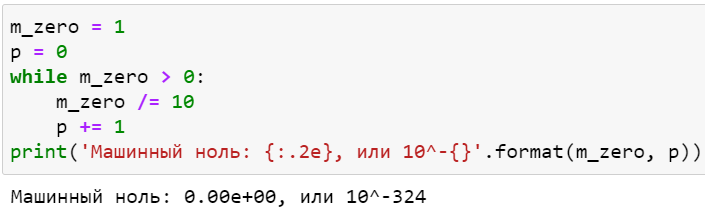
\includegraphics{m_zero.png}

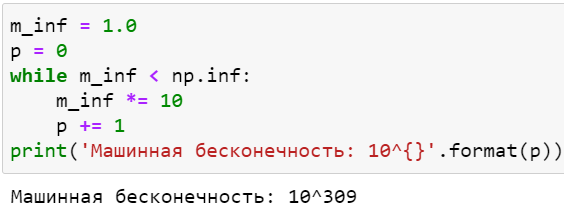
\includegraphics{m_inf.png}

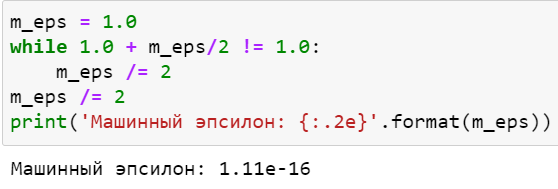
\includegraphics{m_eps.png}
\newpage

\section*{Задача 1.2}

\subsection*{Постановка задачи}
Исследовать поведение погрешности приближения функции $F(x)$ частичными суммами на отрезке $[a, b]$
\[
	F(x) = e^x + \cos x, [-2, 2]
\]

\subsection*{Решение}
Получим разложение функции $F(x)$ в ряд Тейлора в окрестности нуля:
\[
	F(x) = \sum\limits_{n=0}^{\infty}\frac{x^n}{n!} + \sum\limits_{n=0}^{\infty}\frac{(-1)^n \cdot x^{2n}}{(2n)!} = 2 + \frac{x}{1!} + \frac{x^3}{3!} + \frac{2x^4}{4!} + \frac{x^5}{5!} + \frac{x^7}{7!} + \frac{2x^8}{8!} \ldots
\]
Напишем подпрограммы для вычисления функции $f(x)$ и $n$-ых частичных сумм разложения и построим их график и график абсолютных погрешностей. (Весь код программы и графики представлены в файле "source.pdf")

\noindent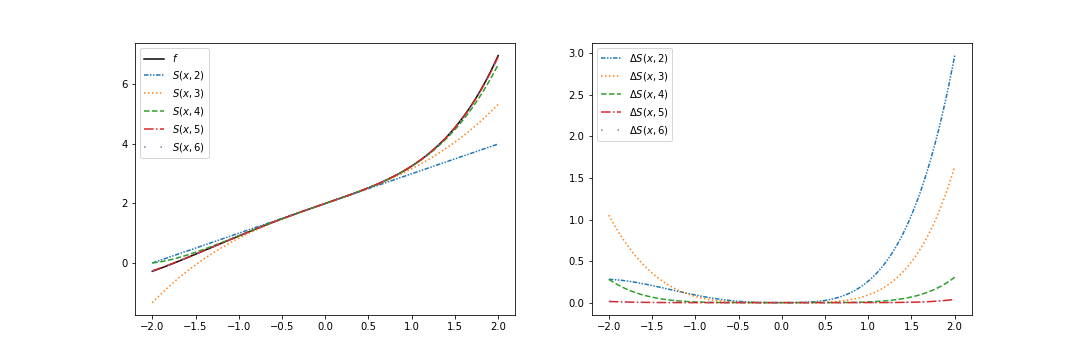
\includegraphics[width=18cm]{output_7_1.png}

Определив номер частичной суммы(6), относительная погрешность которой меньше машинного эпсилон, построим графики погрешностей и сравним их с графиками погрешностей, полученных после округления до 3-х разрядов мантиссы.

Вот графики погрешностей без округления:\newline
\noindent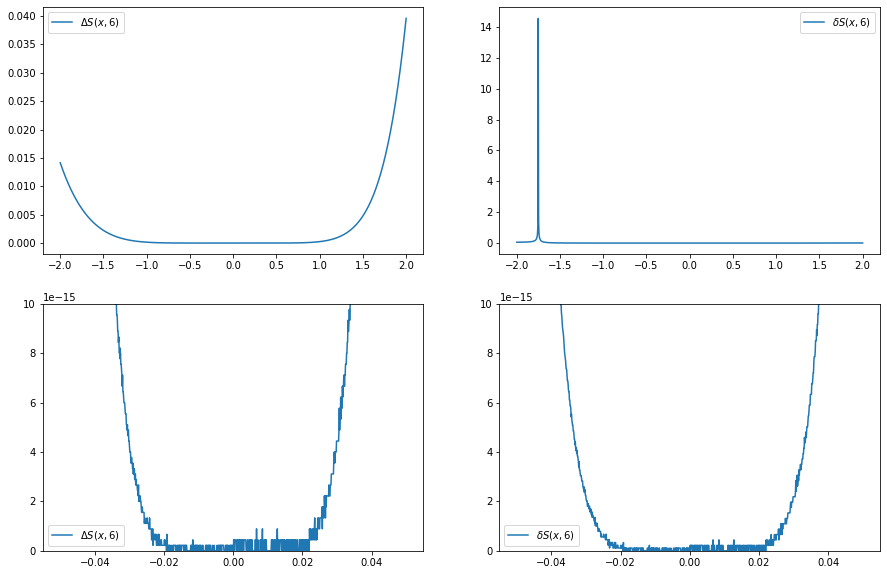
\includegraphics[width=17cm]{output_9_1.png}

А вот абсолютная и относительные погрешности частичной суммы  $S(x, 6)$ с округлением до 3-х разрядов мантиссы.\newline
\noindent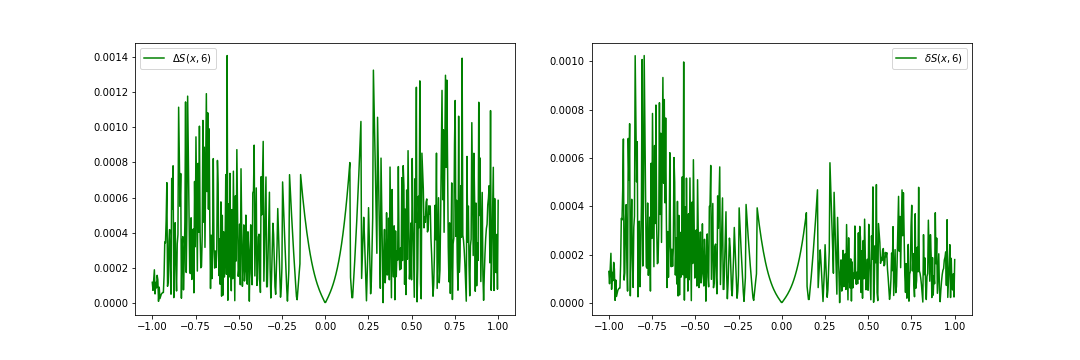
\includegraphics[width=19cm]{output_12_1.png}

Можно заметить, что в случае без округления, относительная погрешность на отрезке $[-0.04, 0.04]$ находится в пределах от $10^{-16}$(то есть машинного эпсилон) до $10^{-14}$, когда в случае с округлением колебания происходят в пределах от $10^{-4}$ до $10^{-3}$.

\newpage
\section*{Задача 1.3}
\subsection*{Постановка задачи}

Дана функция $f(a, b, c)$. Значения переменных указаны в варианте со всеми верными цифрами. Оценить погрешность результата двумя способами: а) используя оценки погрешности для арифметических операций, б) используя общую формулу погрешностей. Результат представить в двух формах записи: с явным указанием погрешностей и с учетом количества верных цифр.

\begin{gather*}
	f(x) = \frac{a + b}{b - c}\\
	a = 52.31\\
	b = 48.95\\
	c = 47.81
\end{gather*}

\subsection*{Решение 1 (с оценкой погрешности для арифметических операций)}

Значение функции - 88.824561403 \newline
Сначала запишем абсолютные погрешности входных данных и расчитаем относительные:

\begin{gather*}
	\Delta a =\Delta b = \Delta c = 0.005 \\
	\delta a = \Delta a / a = 0.005 / 52.31 = 0.000095584\\
	\delta b = \Delta b / b  = 0.005 / 48.95 = 0.000102145\\
	\delta c = \Delta c / c = 0.005 / 47.81 = 0.000104581\\
\end{gather*}

Для вычисления погрешности функции используем формулы погрешности арифметических операций:
\begin{gather*}
	\Delta(a + b) = \Delta(b - c) \leq 0.005 + 0.005 = 0.01\\
	\delta(a + b) = \Delta(a + b) / (a + b) = 0.000098756\\
	\delta(b - c) = \Delta(b - c) / (b - c) = 0.008771929\\
	\delta((a + b)/(b - c)) \leq \frac{\delta(a + b) + \delta(b - c)}{1 - \delta(b - c)} = 0.008949187 = \delta f
\end{gather*}
Отсюда: $ \Delta f = 0.008949187 \cdot 88.824561403 = 0.794907610$

\newpage
\subsection*{Решение 2 (с общей формулой погрешности)}

Вычислим частные производные функции $f(a, b, c)$:
\begin{gather*}
	\frac{\delta f}{\delta a} = \frac{1}{b - c} = 0.877192982\\
	\frac{\delta f}{\delta b} = \frac{(b-c) - (a + b)}{(b-c)^2} = -77.039088950\\
	\frac{\delta f}{\delta c} = \frac{a + b}{(b-c)^2} = 77.916281933
\end{gather*}

Тогда по формуле погрешности функции нескольких переменных получим:
\newline
$\Delta f = 0.877192982\cdot0.005 + 77.039088950\cdot0.005 + 77.916281933\cdot0.005 = 0.779162819$

Тогда относительная погрешность составит: $\delta f = \Delta f / f = 0.779162819 / 88.824561403 = 0.008771930$

Таким образом мы получили что, использовав оценку сверху относительной погрешности для арифметических операций, мы  получили результат, отличающийся от полученного с помощью общей формулы на $0.008949187 - 0.008771930 = 0.000177257$
\newline
Ответ: $f(52.31, 48.95, 47.81) = 88.8 \pm 0.8$, то есть имеем результат с двумя верными цифрами.
\end{document}